\documentclass{article}
\usepackage[utf8]{inputenc}
\usepackage{listings}
\usepackage{CJKutf8}
\usepackage{amsmath}
\usepackage{graphicx}
\usepackage[export]{adjustbox}
\usepackage{tikz}
\usetikzlibrary{trees,automata, positioning, arrows}

\tikzset{
->, % makes the edges directed
>= stealth, % makes the arrow heads bold
node distance=5cm, % specifies the minimum distance between two nodes. Change if necessary.
every state/.style={thick, fill=gray!10}, % sets the properties for each ’state’ node
initial text=$ $, % sets the text that appears on the start arrow
}

\tikzstyle{lightedge}=[blue]
\tikzstyle{mainedge}=[red,very thick]
\tikzstyle{inputBit}=[rectangle,fill=red, text=white]
\tikzstyle{outputBit}=[rectangle,fill=blue, text=white]
\tikzstyle{pointer}=[orange,->,dashed]


\newcommand{\trellisEdges}[4]{
    \newcounter{ctra}
    \setcounter{ctra}{#3}%
    \ifodd\value{ctra}
        \draw[lightedge] (s#1) -- node[above, black, font=\scriptsize] {#4} (s#2) ;
    \else
        \draw[mainedge] (s#1) --  node[above, black, font=\scriptsize] {#4} (s#2);
    \fi%
}

% #1=x; #2=y; #3=In; #4=Out
\newcommand{\trellisInOut}[4]{
    \node[inputBit] (in#1) at (#1+0.5,5) {#3};
    \node[outputBit] (out#1) at (#1+0.5,6) {#4};
    \draw[pointer] (in#1) -- (#1+0.5,#2);
}

\title{Lab5 Report}
\author{b09901142 EE3 呂睿超}
\date{November 2022}

\usepackage{xcolor}

\definecolor{codegreen}{rgb}{0,0.6,0}
\definecolor{codegray}{rgb}{0.5,0.5,0.5}
\definecolor{codepurple}{rgb}{0.58,0,0.82}
\definecolor{backcolour}{rgb}{0.8,0.9,0.8}

\lstdefinestyle{mystyle}{
    backgroundcolor=\color{backcolour},   
    commentstyle=\color{codegreen},
    keywordstyle=\color{magenta},
    numberstyle=\tiny\color{codegray},
    stringstyle=\color{codepurple},
    basicstyle=\ttfamily\footnotesize,
    breakatwhitespace=false,         
    breaklines=true,                 
    captionpos=b,                    
    keepspaces=true,                 
    numbers=left,                    
    numbersep=5pt,                  
    showspaces=false,                
    showstringspaces=false,
    showtabs=false,                  
    tabsize=2
}

\lstset{style=mystyle}

\begin{document}
\begin{CJK*}{UTF8}{bsmi}
\maketitle

\section{Analysis of Convolutional Codes}
\quad \textbf{g}^{(1)} = [1,0,1],  \quad \textbf{g}^{(2)} = [1,1,1]  
\subsection{(a)}
\begin{enumerate}
    \item Observe that there is only a group of g(FIR coefficients), implies that k = 1
    \item Observe that there are two g, implies that n = 2(it generates to coded bits from 1 input bit)
    \item Therefore, R(code rate) = $\frac{k}{n} = \frac{1}{2}$
\end{enumerate}


\subsection{(b)}
   \begin{figure}[h]
    \centering
    \includegraphics[width=0.8\textwidth]{IMG_0150.jpg}
    \caption{\label{fig:IMG_0150.png} The shift register structure of\emph{question 1}}
    \end{figure}

\subsection{(c)}
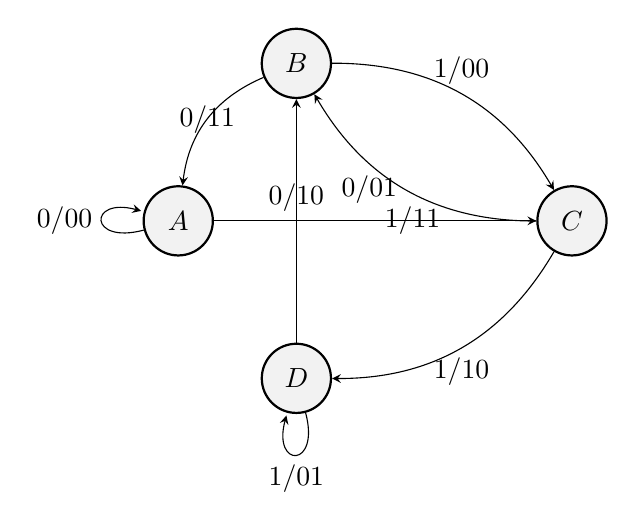
\begin{tikzpicture}
\node[state] (q1) {$A$};
\node[state] at (1.5,2) (q2) {$B$};
\node[state, right of=q1] (q3) {$C$};
\node[state] at (1.5,-2) (q4) {$D$};
\draw (q1) edge[loop left] node{0/00} (q1)
    (q1) edge[right] node{1/11} (q3)
    (q2) edge[bend right] node{0/11} (q1)
    (q2) edge[bend left, above] node{1/00} (q3)
    (q3) edge[bend left, below,left = 0.1] node{0/01} (q2)
    (q3) edge[bend left, below] node{1/10} (q4)
    (q4) edge[above] node{0/10} (q2) 
    (q4) edge[loop below] node{1/01} (q4);
\end{tikzpicture}

The figure above is the state transition diagram. The input and output of each transition is shown in the format as 'input($b_i$)/output($c_i^{(1)}c_i^{(2)}$)'

\subsection{(d)}
\begin{tikzpicture}[x=1.5cm, y=-1cm]
    \node at (-0.5,0) [left] {$A=00$};
    \node at (-0.5,1) [left] {$B=01$};
    \node at (-0.5,2) [left] {$C=10$};
    \node at (-0.5,3) [left] {$D=11$};

    % Nodes
    \foreach \x in {0,...,5} {
        \node at (1.5*\x,-.7) {$t=\x$};
        \foreach \y in {0,...,3} {
            \node (s\x\y) at (1.5*\x,\y) [circle,fill=blue] {};
        }
        
    }

    % Edges
    \trellisEdges{00}{10}{0}{$00$}
    \trellisEdges{00}{12}{1}{$11$}
    \trellisEdges{10}{20}{0}{$00$}
    \trellisEdges{10}{22}{1}{$11$}
    \trellisEdges{12}{21}{0}{$01$}
    \trellisEdges{12}{23}{1}{$10$}
    
    \trellisEdges{20}{30}{0}{$00$}
    \trellisEdges{20}{32}{1}{$11$}
    \trellisEdges{21}{30}{0}{$11$}
    \trellisEdges{21}{32}{1}{$00$}
    \trellisEdges{22}{31}{0}{$01$}
    \trellisEdges{22}{33}{1}{$10$}
    \trellisEdges{23}{31}{0}{$10$}
    \trellisEdges{23}{33}{1}{$01$}
    
    \trellisEdges{30}{40}{0}{$00$}
    \trellisEdges{30}{42}{1}{$11$}
    \trellisEdges{31}{40}{0}{$11$}
    \trellisEdges{31}{42}{1}{$00$}
    \trellisEdges{32}{41}{0}{$01$}
    \trellisEdges{32}{43}{1}{$10$}
    \trellisEdges{33}{41}{0}{$10$}
    \trellisEdges{33}{43}{1}{$01$}
    
    \trellisEdges{40}{50}{0}{$00$}
    \trellisEdges{40}{52}{1}{$11$}
    \trellisEdges{41}{50}{0}{$11$}
    \trellisEdges{41}{52}{1}{$00$}
    \trellisEdges{42}{51}{0}{$01$}
    \trellisEdges{42}{53}{1}{$10$}
    \trellisEdges{43}{51}{0}{$10$}
    \trellisEdges{43}{53}{1}{$01$}
    

    % Inputs and Outputs
    %\node at (-0.5,5) [left] {Input Bits};
    %\node at (-0.5,6) [left] {Output Bits};

    %\trellisInOut{0}{0.5}{1}{11}
    %\trellisInOut{1}{2.0}{1}{01}
    %\trellisInOut{2}{2.5}{0}{01}
\end{tikzpicture}

\subsection{(e)}
\begin{tikzpicture}[x=1.5cm, y=-1cm]
    \node at (-0.5,0) [left] {$A=00$};
    \node at (-0.5,1) [left] {$B=01$};
    \node at (-0.5,2) [left] {$C=10$};
    \node at (-0.5,3) [left] {$D=11$};

    % Nodes
    \foreach \x in {0,...,7} {
        \node at (\x,-.7) {$\x$};
        \foreach \y in {0,...,3} {
            \node (s\x\y) at (\x,\y) [circle,fill=blue] {};
        }
        
    }
    \trellisEdges{00}{10}{0}{$00$}
    \trellisEdges{10}{22}{1}{$11$}
    \trellisEdges{22}{31}{0}{$01$}
    \trellisEdges{31}{42}{1}{$00$}
    \trellisEdges{42}{51}{0}{$01$}
    
    \trellisEdges{51}{62}{1}{$00$}
    \trellisEdges{62}{71}{0}{$01$}
    


\end{tikzpicture}
\begin{enumerate}
    \item Using Viterbi's algorithm to determine the path, I got the following result.
    \item The decoded codewords $\mathbf{\hat{c}}$ = \{$\hat{c}_i$\} = [0 0 1 1 0 1 0 0 0 1 0 0 0 1]
    \item The decoded bits $\mathbf{\hat{b}}$ = \{$\hat{b}_i$\} = [0 1 0 1 0 1 0]
\end{enumerate}
\subsection{(f)}
\quad From \emph{question 1e}, the Hamming distance is (d(y,$\mathbf{\hat{c}}$)) = 2


\section{Implementation of Convolutional Code #1}
\subsection{(a)} 
\begin{enumerate}
    \item Following the instructions, I implemented the convolutional encoder.
    
    \item Following the hint, I generate a finite state table(FSM\_table). An example of the FSM\_table is as following,
    
    \begin{figure}[h]
    \centering
    \includegraphics[width=0.8\textwidth]{FSM_table.png}
    \caption{\label{fig:FSM_table.png} An example of FSM\_table}
    \end{figure}
        \begin{enumerate}
            \item The first column of the figure is $b_i$,which is the incoming bit.
            \item The second column of the figure is $b_{i-1}b_{i-2}$,which is the stored bits in the buffer.
            \item The next few columns are the encoded bits($c_i$). I used a buffer(temp\_buf) to simulate the bit incoming process, and used xor functions to get the encoded results.
            \item The last column is the new state(state after state transition).
        \end{enumerate}
    
    
    \item I used strcmp function to check the current state from the processing buffer. And look up the generated FSM\_table to find the correct encoded results.
    \item The encoded bits of the example \textbf{b} = [1 0 1 1 0] is 
    
    \textbf{c} = [1     1     1     0     0     1     1     0     0     1     1     0     0     1     0]

    
\end{enumerate}

\subsection{(b)}
\begin{enumerate}
    \item The FSM\_table also has to be generated in the decoding process in order to look up. 
    \item I generated a state transition diagram to look up the relationships between states.
    \begin{figure}[h]
    \centering
    \includegraphics[width=0.8\textwidth]{state_trans.png}
    \caption{\label{fig:state_trans.png} An example of state transition diagram}
    \end{figure}
        \begin{enumerate}
            \item The first column indicates the current state.
            \item The second column indicates the resulting state if incoming bit is '0'.
            \item The next column indicates the resulting state if incoming bit is '1'.
            \item The fourth column indicates the generated encoding bits if incoming bit is '0'.
            \item The last column indicates the generated encoding bits if incoming bit is '1'.
        \end{enumerate}
    
    \item Next, I generated a trellis\_diagram to implement \textbf{Viterbi's Algorithm}.
    \begin{figure}[h]
    \centering
    \includegraphics[width=1.1\textwidth]{trellis_diag.png}
    \caption{\label{fig:trellis_diag.png} An example of Trellis diagram}
    \end{figure}
        \begin{enumerate}
            \item The first number of each cell is the current minimum cost of all possible path reaching that node.
            \item The second number of each cell is the previous node of the chosen minimum cost path
            \item I generated this diagram by iterating through all cells from left to right from up to down. (By filling the cells and holding the minimum cost)
        \end{enumerate}
    \item Last, I follow the path from the last cell
    
    (trellis\_table\{size(trellis\_table,2),1\} ) to the first cell(because only reversed traversing can determine the only chosen path.)
    \item Next, I reverse the resulting path(turning back to the original order). Finally, look up the state transition diagram to generate the final decoded data
    \item The decoded bits of the example \textbf{d} = [0 1 0 0 0 0 1 0 1 1 1 1 0 0 1 0 1 1 0 0 0] is \textbf{b} = [0     0     0     1     0     0     0] 
    \item The snapshot of the matlab program of the result of the example(corresponding to 2.2.4\&2.3.6) is in \emph{Appendix 1} , which both verifies the ideal result.
\end{enumerate}

\subsection{(c)}
\begin{enumerate}
    \item I used random seed to determine the input bitstring.
    \item Apply the convolutional encoder.
    \item I also used random seed and compare it with p. If seed < p, means that it is in the probability that the noise is occurred. Thus, flip the bit as if it goes through a simulating noisy channel.
    \item Apply the convolutional decoder. 
    \item The plot of the simulation results is as the figure below
    \begin{figure}[h]
    \centering
    \includegraphics[width=0.9\textwidth]{2c.jpg}
    \caption{\label{fig:2c.png}the simulation results of \emph{question 2c}}
    \end{figure}
    \item Observations of this figure are as below
        \begin{enumerate}
            \item As p increases, the BER increases as intuition.(Noisier channel rises error rate.)
            \item When p $>$  0.5, BER $>$ 0.5. Which means that the decoded can't recover the error correctly an that the output bit is unreliable.
        \end{enumerate}
\end{enumerate}


\section{Implementation of Convolutional Code \#2}
\begin{enumerate}
    \item Change the impulse response to impulse\_response\_c = [1,1,0;1,0,1];
    \item The plot of the simulation results is as the figure below
    \begin{figure}[h]
    \centering
    \includegraphics[width=0.9\textwidth]{3.jpg}
    \caption{\label{fig:3.png}the simulation results of \emph{question 3}}
    \end{figure}
    \item A major difference between \emph{question 2c} and \emph{question 3} is that it seems to converge at BER = 0.5 while p increases.
    \item The reason the leads to it is that if a certain $c_i$ with length = 2 has both bit flipped because of the interruption of the noisy channel, the Viterbi's Algorithm tends to choose either of the decoded bit with \textbf{equal possibility}(cost of each choice = 1). The \textbf{"equal possibility"} implies the result of BER = 0.5.
    
\end{enumerate}


\section{Appendix}
\subsection{the resulting encoded/decoded bits of \emph{question 2}}
\begin{figure}[h]
\centering
\includegraphics[width=0.9\textwidth]{result2.png}
\caption{\label{fig:result2.png}the resulting encoded/decoded bits of \emph{question 2}}
\end{figure}

\end{CJK*}
\end{document}
